\documentclass[10pt]{beamer}

\usepackage{amsfonts}
\usepackage{subfiles}
\usepackage[T2A]{fontenc}
\usepackage[utf8]{inputenc}
\usepackage[russian]{babel}

\usepackage{amsmath, amsfonts, amssymb, amsthm, mathtools, mathrsfs}
\usepackage{wasysym, dsfont}
\usepackage{graphicx}
\usepackage{float}
\usepackage{wrapfig}

\usepackage{caption}
\usepackage{subcaption}
\usepackage{longtable}
% \usepackage{subfigure}

\usepackage{multicol}
\DeclareMathOperator*{\argmax}{\arg\!\max}
\DeclareMathOperator*{\argmin}{\arg\!\min}

\mode<presentation>
{
	\usetheme{boxes}
	\beamertemplatenavigationsymbolsempty
	
	\setbeamertemplate{footline}[page number]
	\setbeamersize{text margin left=1.5em, text margin right=2.0em}
}
\newcommand\blfootnote[1]{%
	\begingroup
	\renewcommand\thefootnote{}\footnote{#1}%
	\addtocounter{footnote}{-1}%
	\endgroup
}
\newcommand\FontUP{\fontsize{12}{12}\selectfont}


\title[]{Лабораторная работа 207}
\author{Охотников Никита Владимирович}
\institute{МФТИ}
\date{2024}


\begin{document}

\begin{frame}
  \titlepage
\end{frame}


\begin{frame}
	\frametitle{Введение}
	\begin{block}{Цели}
		\begin{itemize}
			\item Рассмотреть обобщение SVD на тензоры размерности 4 -- алгоритм HOSVD
			\item Использовать trunctated SVD для полученных разложений по аналогии с двумерным PCA для уменьшения размера хранимого представления
			\item Оценить качество восстановления 4-хмерных видео при снижении одной из размерностей в разложении до единицы
		\end{itemize}
	\end{block}	
\end{frame}

\begin{frame}
	\frametitle{Теоретическая часть}
	\begin{block}{Tucker decomposition}
		На примере трехмерного тензора, для понятной визуализации разложение Таккера выглядит следующим образом:
		$$\mathbf{\underline{X}} \in \mathbb{R}^{I \times J \times K}, ~~\mathbf{A} \in \mathbb{R}^{I \times Q}, ~~\mathbf{B} \in \mathbb{R}^{J \times R}, ~~\mathbf{C} \in \mathbb{R}^{K \times P}$$
			\begin{center}
				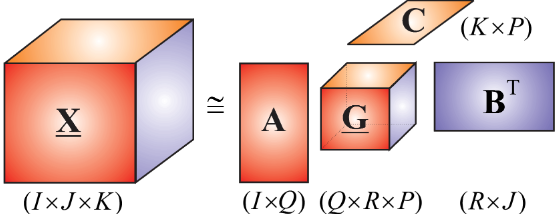
\includegraphics[scale =0.65]{./tucker.png}
			\end{center}
		$$\mathbf{\underline{X}}\simeq \sum_{q=1}^{Q} \sum_{r=1}^{R} \sum_{p=1}^{P} g_{qrp} \mathbf{a}_q \circ \mathbf{b}_r \circ \mathbf{c}_p = \mathbf{\underline{G}} \times_1 \mathbf{A} \times_2 \mathbf{B} \times_3 \mathbf{C} = \Big[ \mathbf{\underline{G}};  \mathbf{A},  \mathbf{B}, \mathbf{C}   \Big]$$
	\end{block}	
\end{frame}

\begin{frame}
	\frametitle{Теоретическая часть}
	\begin{block}{Higher Order Singular Value Decomposition (HOSVD)}
		HOSVD -- специальный случай разложения Таккера, в котором все фактор-матрицы ортогональны. Фактор матрицы находятся как матрицы из truncated-SVD для разверток $X$ по соответствующей моде. Для трехмерного случая выше:
		$$\mathbf{X}_{(1)} = \mathbf{U}_1 \Sigma_1 \mathbf{V}_1^T \quad \rightarrow \quad \mathbf{A} = \mathbf{U}_1[1:R_1]$$
		$$\mathbf{X}_{(2)} = \mathbf{U}_2  \Sigma_2 \mathbf{V}_2^T \quad \rightarrow \quad \mathbf{B} = \mathbf{U}_2[1:R_2]$$
		$$\mathbf{X}_{(3)} = \mathbf{U}_3  \Sigma_3 \mathbf{V}_3^T \quad \rightarrow \quad \mathbf{C} = \mathbf{U}_3[1:R_3]$$
		Core-тензор после этого вычисляется как
		$$\mathbf{\underline{G}} = \mathbf{\underline{X}} \times_1 \mathbf{A}^T \times_2 \mathbf{B}^T \times_3 \mathbf{C}^T $$

	\end{block}	
\end{frame}

\begin{frame}
	\frametitle{Практическая часть часть}
	\begin{block}{Данные}
		В качестве синтетического датасета рассмотрим собственноручно сгенерированный ColoredMovingMnist -- пары семплов из MNIST \footnote{http://yann.lecun.com/exdb/mnist/} случайного цвета, двигающиеся на черном фоне в произвольных направлениях в течение 4 секунд. \\
		Исходный размер $20\times 40 \times 40 \times 3$.
		Рассматривается сжатие по времени до $[1, 5, 10]$, по высоте и ширине до $[5, 10, 20]$ и по каналам до $[1, 2]$
	\end{block}	
	\begin{figure}
		\centering
		
\includegraphics[scale =0.35]{./sample2.png}
	\end{figure}
\end{frame}



\begin{frame}
	\frametitle{Результаты эксперимента}
		\centering
		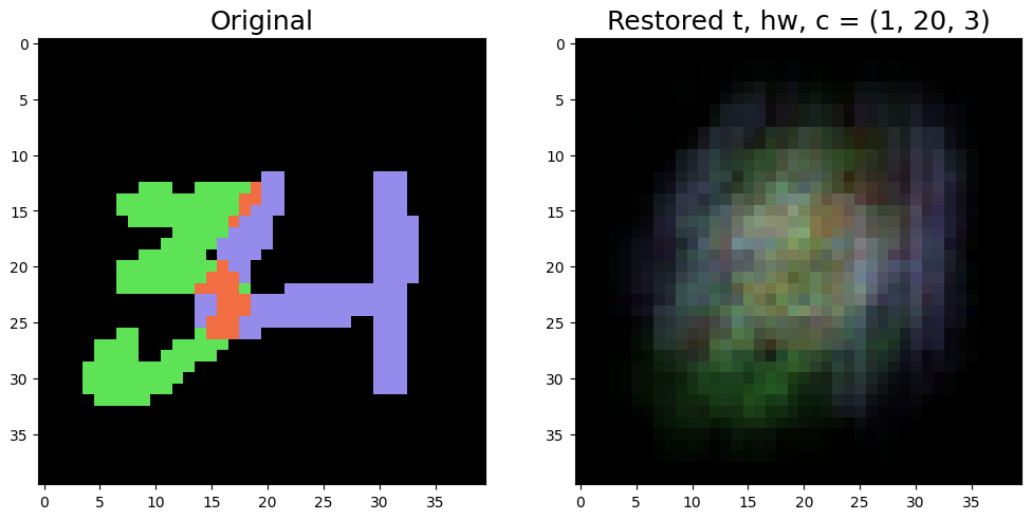
\includegraphics[scale=0.35]{./res1_20_3.png}
		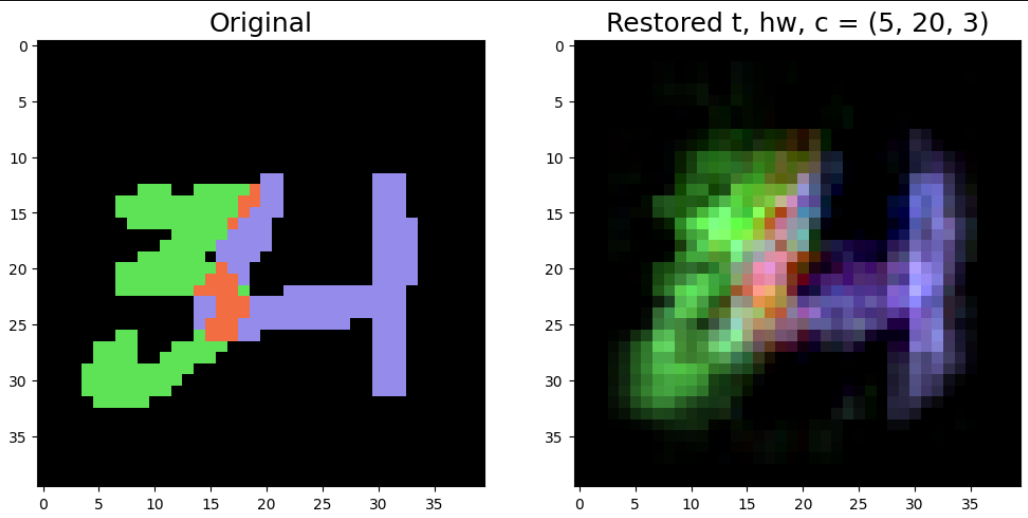
\includegraphics[scale=0.35]{./res5_20_3.png}
\end{frame}

\begin{frame}
	\frametitle{Результаты эксперимента}
	\centering
	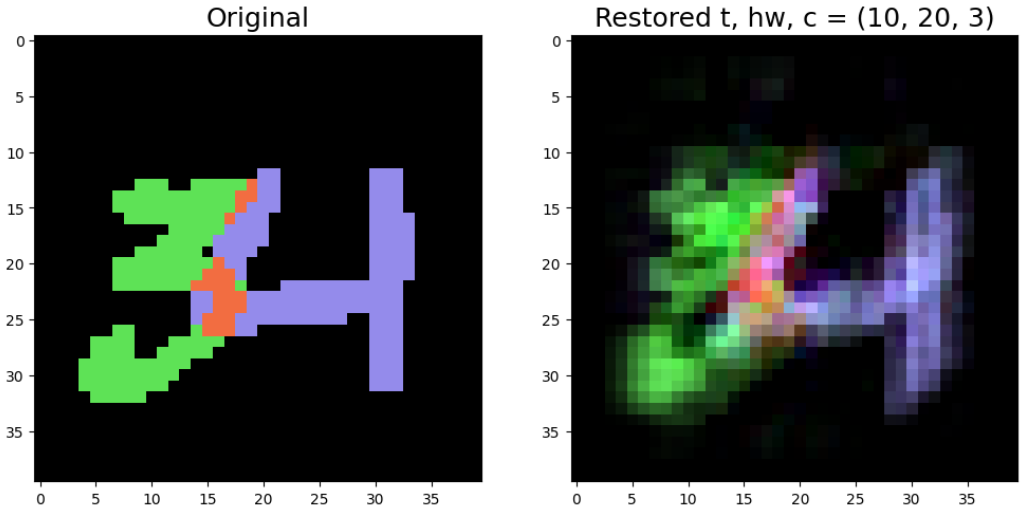
\includegraphics[scale=0.35]{./res10_20_3.png}
	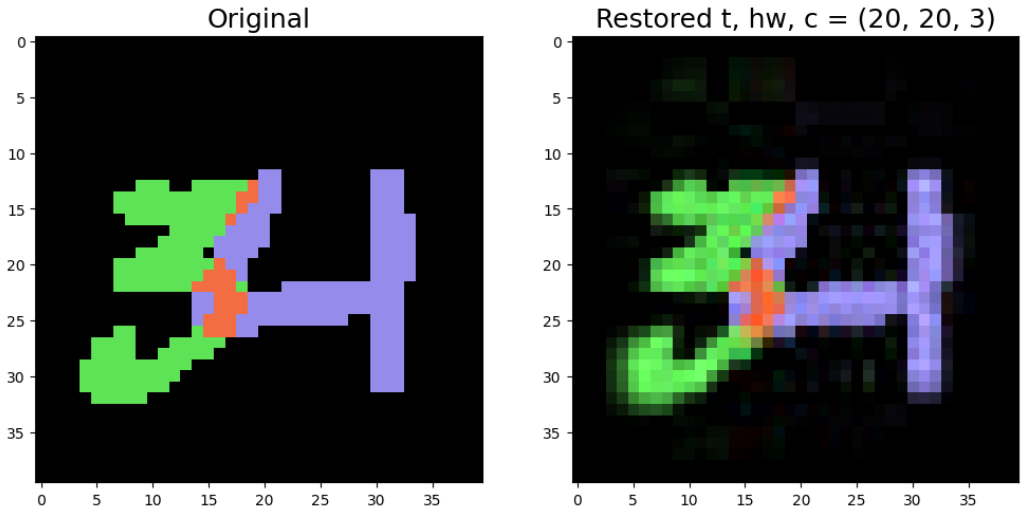
\includegraphics[scale=0.35]{./res20_20_3.png}
\end{frame}

\begin{frame}
	\frametitle{Результаты эксперимента}
	\centering
	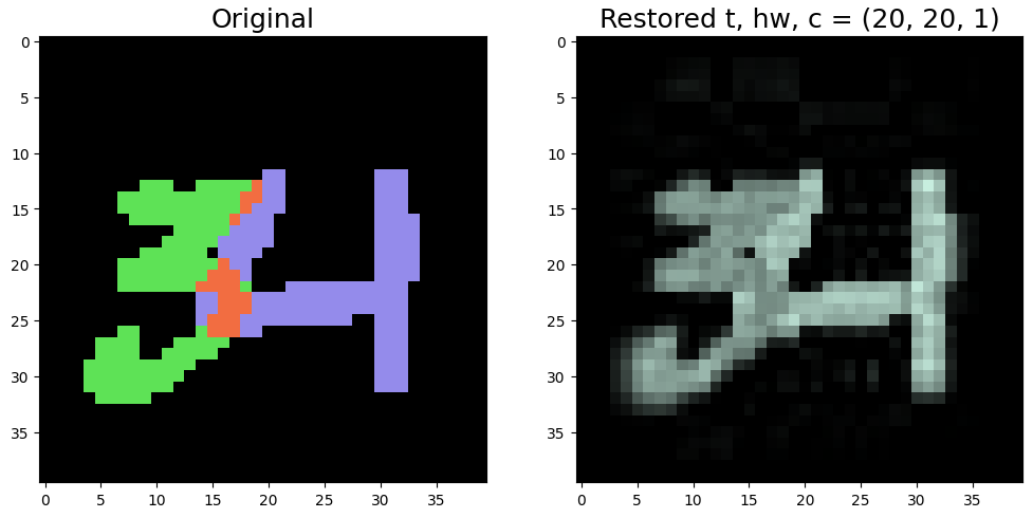
\includegraphics[scale=0.35]{./res20_20_1.png}
	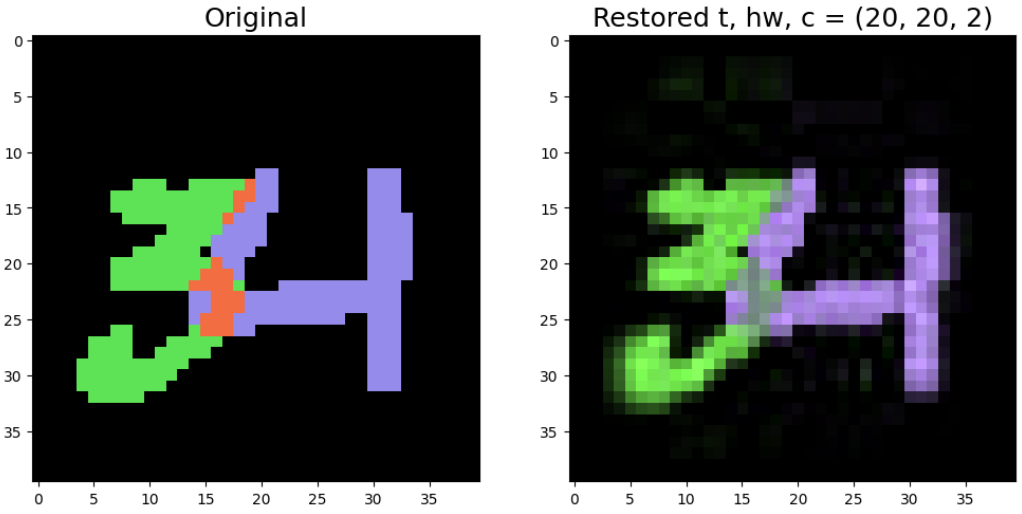
\includegraphics[scale=0.35]{./res20_20_2.png}
\end{frame}


\begin{frame}
	\frametitle{Результаты эксперимента}
	\begin{block}{Зависимость ошибки от compression rate}
		\centering
		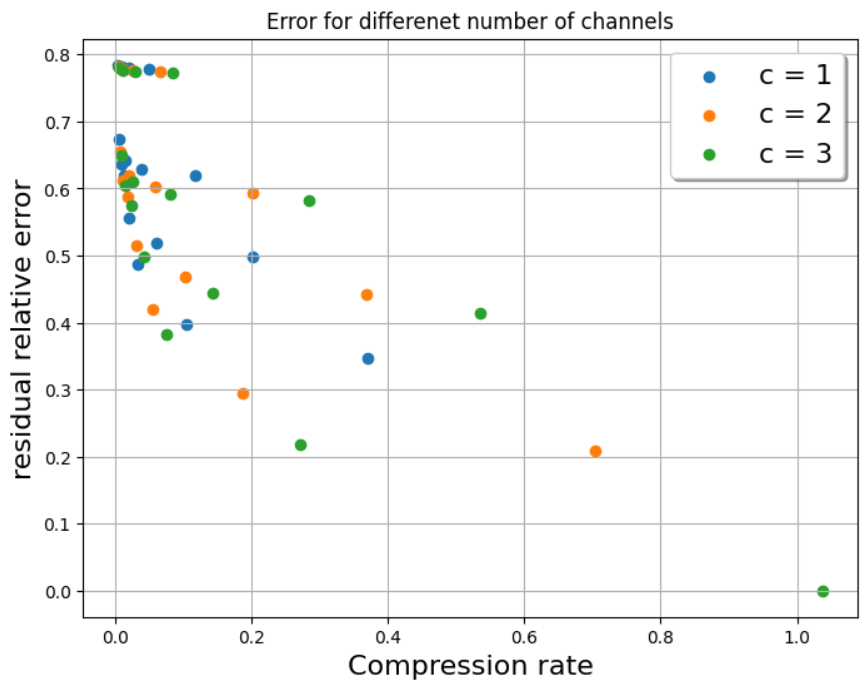
\includegraphics[scale=0.45]{./channels.png}
	\end{block}		
\end{frame}

\begin{frame}
	\frametitle{Результаты эксперимента}
	\begin{block}{Зависимость ошибки от compression rate}
		\centering
		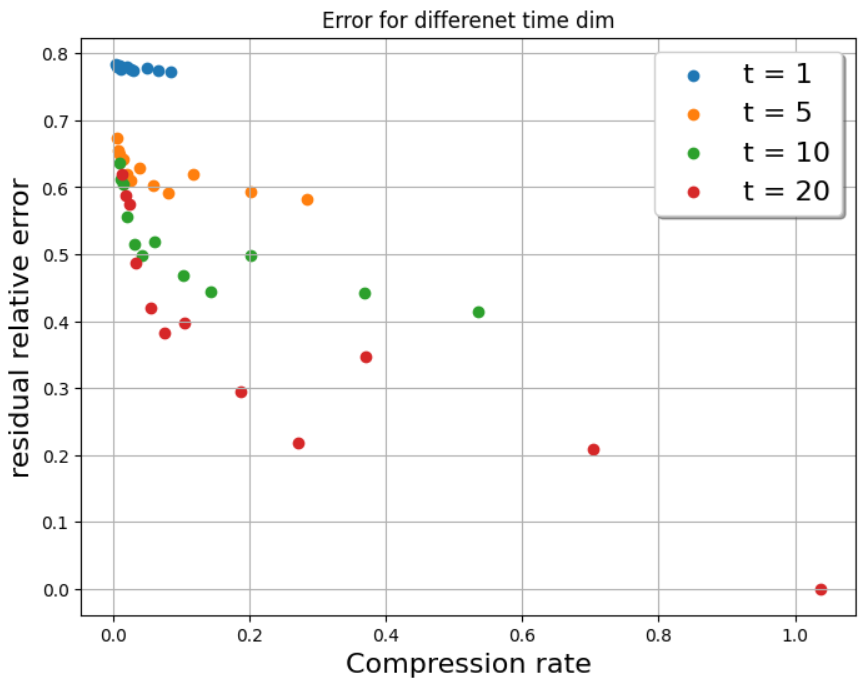
\includegraphics[scale=0.45]{./time.png}
	\end{block}		
\end{frame}

\begin{frame}
	\frametitle{Результаты эксперимента}
	\begin{block}{Grayscale}
		\centering
		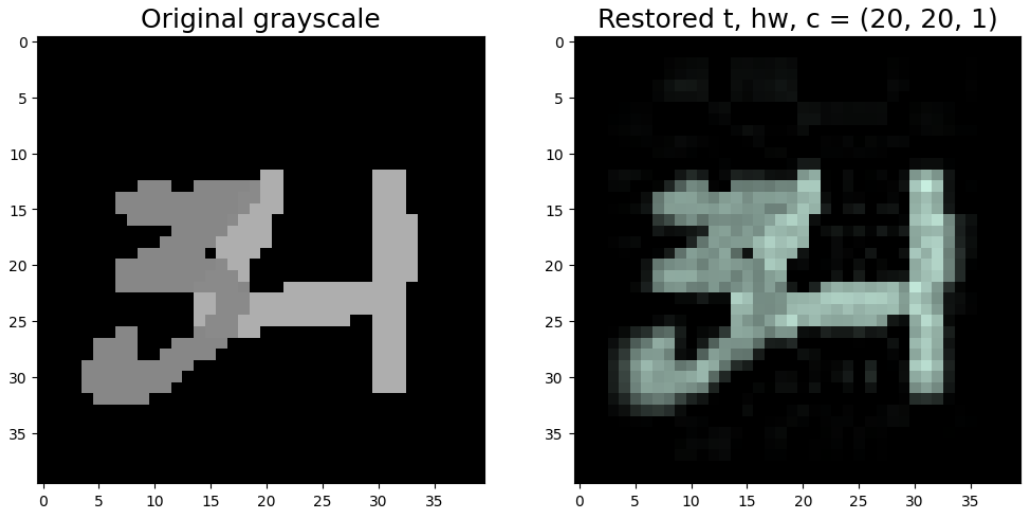
\includegraphics[scale=0.45]{./grayscale.png}
	\end{block}		
\end{frame}

\begin{frame}
	\frametitle{Заключение}
	\begin{block}{Выводы}
		\begin{itemize}
		\item Метод работает
		\item Метод едва ли позволяет значительно сжать видео рассмотренного размера, поскольку вместо одного тензора приходится хранить четыре
		\item избавиться от целой размерности можно только по размерности каналов
		\item Сжатие по размерности каналов до одного сравнимо с ручным по яркости
		\end{itemize}
	\end{block}		
\end{frame}

\end{document}
